% Source: https://tex.stackexchange.com/a/203259/6880

\documentclass[tikz, border=5mm]{standalone}
\usetikzlibrary{calc, chains, decorations.pathmorphing}

\begin{document}
 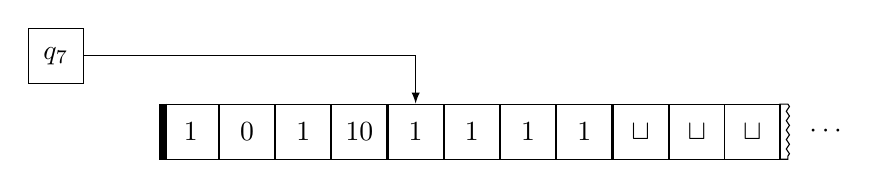
\begin{tikzpicture}
  \tikzset{tape/.style={minimum size=.7cm, draw}}
  \begin{scope}[start chain=0 going right, node distance=0mm]
   \foreach \x [count=\i] in {1,0,1,10,1,1,1,1,$\sqcup$,$\sqcup$,$\sqcup$} {
    \ifnum\i=11 % if last node reset outer sep to 0pt
      \node [on chain=0, tape, outer sep=0pt] (n\i) {\x};
      \draw (n\i.north east) -- ++(.1,0) decorate [decoration={zigzag, segment length=.12cm, amplitude=.02cm}] {-- ($(n\i.south east)+(+.1,0)$)} -- (n\i.south east) -- cycle;
     \else
      \node [on chain=0, tape] (n\i) {\x};
     \fi
     \ifnum\i=1 % if first node draw a thick line at the left
      \draw [line width=.1cm] (n\i.north west) -- (n\i.south west);     
     \fi
   }
   \node [right=.25cm of n11] {$\cdots$};
   \node [tape, above left=.25cm and 1cm of n1] (q7) {$q_7$};
   \draw [>=latex, ->] (q7) -| (n5); 
  \end{scope}  
 \end{tikzpicture}
\end{document} 